\section{Vergelijkingsoverzicht}
\label{sec:evaluatie-spinnenweb}

% eerst de grafiek van onze initiële criteria en formules
% sander 

% besluiten  (de getallen zijn geen procenten)
% 1) Kendo: 1,51 
% 2) Lungo: 1,14
% 3) jQM: 1,03
% 4) ST: 0,62

% but...
% kendo is winnaar (uitstekend op pop, gebruik en ondersteuning % Waarom kiezen voor kendo:
% - architectuur => minder productief maar meer bruikbaar
% - hoge licentiekost => professionele support. Ondanks niet open source toch populiar (meest populair)
% + native look-and-feel => laadtijden stijgen?  meer op native applicatie (positieve impact niet geevalueerd) (iOS lay-out sterk gelijkend op
%echte iOS,  Android minder gelijkend, Blackberry en windows niet bekeken)

% tweede is lungo % Waarom kiezen voor lungo:
% - productiviteit => verkeerde indruk (zonder voorkennis / sumire documentatie maakt het moeilijk)
% - support => niet bij oudere android OS (2.3) X)(marktwaarde android 2.3 tov alle devices)X% van de devices vallen dan uit de boot
% + performatie zeer positief => quo js geoptimaliseerd (bedrijf gespecialiseerd in mobile user experience)! (weinig support help hier ook)
% nauwelijks bekend (literatuur, social networks (zie populariteit), ...)

% jQM volgt % Waarom kiezen voor jqm:
% +/- geen architectuur (
    % minder gebruik
    % lagere leercurve (veel HTML, link met js is het lastigst)
    % meer code schrijven (error prone)
% + zeer populair (jQuery core) zie stackoverlow => vragen worden door een hele community opgelost (geen payed support)
% als een easy (geen architectuur) raamwerk + populair (belangrijke klanten,  gekend op social media)

% Sencha (nergens numero uno) % Waar niet kiezen voor st:
% + / - Tools voorhanden (Sencha Cmd / Architect ) om programmeren makkelijker te maken maar tools niet even handig (of betalend)
% - Javascript driven maakt het lastig (alle simple HTML moet in js worden geschreven): meeste lijnen JS + grote bibliotheek => minder performant
% - gebaseerd op webkit => geteste toestellen hadden dit wel (windows phone geen webkit)

%%%%%%%%%%%%%%%%%%%%%%%%%%


% daarna de bindparagraaf door onze 2 improvents (productiviteit en performantie)
% referen naar de nieuwe formules in de respectievelijke secties
% nieuwe formules voor het bereken van het relatieve waarden voor de respectievelijke formules
% tonen van de finale grafiek

\begin{figure}[H]
  \centering
  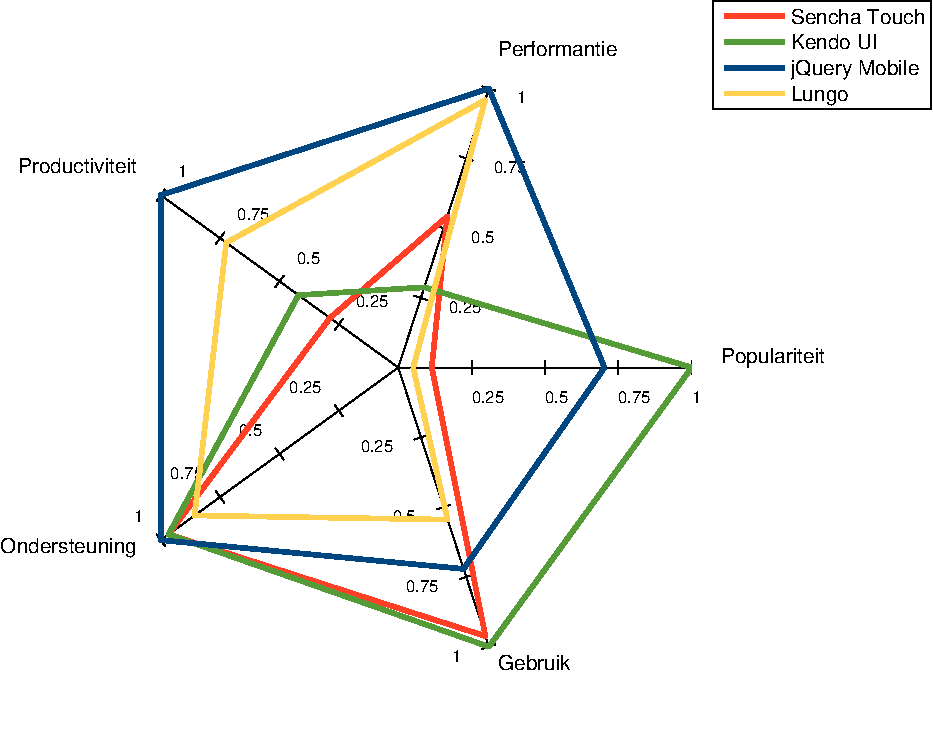
\includegraphics[width=\textwidth]{figuren/spidergraph-final.pdf}
  \caption{Vergelijkingsoverzicht met de vijf vergelijkingscriteria voor \st{},  \kendo{},  \jqm{} en \lungo{}.}
  \label{fig:spinnenweb-final}
\end{figure}

% Finale volgordes (de getallen zijn geen procenten)
% 1) jQM: 1,87
% 2) Kendo: 1,32
% 3) Lungo: 0,88
% 4) ST: 0,73

%nieuwe zaken:
%Productiviteit
  % jqm naar eerste plaats,  andere boeten in (raamwerk met architectuur komen achteraan,  stemt overeen met verwachtingen)
%Performantie:
  %Kendo: iOS crash van lange lijst: performantie daalt van 40% naar 25%
  %Sencha : Performantie verhoogt want gebruikservaring maximaal

%jQM naar eerst plaats, rest schuift een plaats door (buiten st)
% snelle ontwikkeling die performant is en overal ondersteund wordt geen payed support nodig hebt en geen geavanceerde features wil implementeren